%! TEX program = lualatex

%https://docs.google.com/presentation/d/1hQvHxJggiRwQHczaA9fL40V6GM44cOixqQ2S2OEsAhc/edit#slide=id.p

\documentclass[nobackground,dvipsnames,table]{beamer}
\usepackage{tsc}
\usepackage{pdfpc}
\usepackage{pgfpages}
\usepackage{multimedia}

\mode<presentation>
{\usetheme{default}
	\usecolortheme{tsc}
	\setbeamercovered{transparent}
	\useinnertheme[shadow=false]{rounded}
	\usebackgroundtemplate{}
	\setbeamercolor*{frametitle}{parent=palette primary}
	\setbeamerfont{block title}{size={}}
	\setbeamertemplate{navigation symbols}{}
    \setbeamertemplate{itemize items}[circle]
        \setbeamertemplate{enumerate items}[circle]
}

%%%%%%%% edit hyperlink colors %%%%%%%%
\hypersetup{
  colorlinks   = true, 
  urlcolor     = tscurl, % color of external hyperlinks
  linkcolor    = white,   % color of internal links
}

%%% below command addresses log output error when trying to use \\ in \author %%%
\pdfstringdefDisableCommands{%
  \def\\{}%
}

%%%%% the below command allows custom highlights used in this presentation with \hlc %%%%%%
\makeatletter
\let\HL\hl
\renewcommand\hl{%
  \let\set@color\beamerorig@set@color
  \let\reset@color\beamerorig@reset@color
  \HL}
\makeatother

\newcommand{\hlc}[2][yellow]{{%
    \colorlet{foo}{#1}%
    \sethlcolor{foo}\hl{#2}}%
}

\title[]{Emerging Technologies \& Career Advice}
%\subtitle{A document made with thought and care}

\author[]{}
%\institute[TSC]{\large Trust \& Safety Teaching Consortium}
\date[2023]{}
\subject{Trust and Safety}

\AddToShipoutPictureBG*{
  \AtPageLowerLeft{\hspace{-0.4cm}
    
\includegraphics[width=13.1cm]{img/consortium-image}}
}
% Change this to make a file with just slides, just notes or both
%\setbeameroption{hide notes}                 % Only slides
%\setbeameroption{show only notes}            % Only notes
\setbeameroption{show notes on second screen} % Both

\begin{document}

%\coverpage


%%%%%%%%%%%%%%%%%%%%%%%%%%%%%%%%%%%%%%%%%%%%%%%%%%%
%%%%%%%%%%%%%%%%%%%% SLIDE 1 %%%%%%%%%%%%%%%%%%%%%%
%%%%%%%%%%%%%%%%%%%%%%%%%%%%%%%%%%%%%%%%%%%%%%%%%%%
\begin{frame}
    \titlepage
\end{frame}



%%%%%%%%%%%%%%%%%%%%%%%%%%%%%%%%%%%%%%%%%%%%%%%%%%%
%%%%%%%%%%%%%%%%%%%% SLIDE 2 %%%%%%%%%%%%%%%%%%%%%%
%%%%%%%%%%%%%%%%%%%%%%%%%%%%%%%%%%%%%%%%%%%%%%%%%%%
\begin{frame}{Learning Objectives}
\textbf{Today we will:}

\begin{itemize}
    \item Learn about AI/ML, AR/VR, and decentralized systems
    \item Examine how these technologies intersect with Trust \& Safety
    \item Explore career pathways and opportunities
\end{itemize}

\end{frame}



%%%%%%%%%%%%%%%%%%%%%%%%%%%%%%%%%%%%%%%%%%%%%%%%%%%
%%%%%%%%%%%%%%%%%%%% SLIDE 3 %%%%%%%%%%%%%%%%%%%%%%
%%%%%%%%%%%%%%%%%%%%%%%%%%%%%%%%%%%%%%%%%%%%%%%%%%%
\begin{frame}{Emerging Technologies}

\begin{center}
    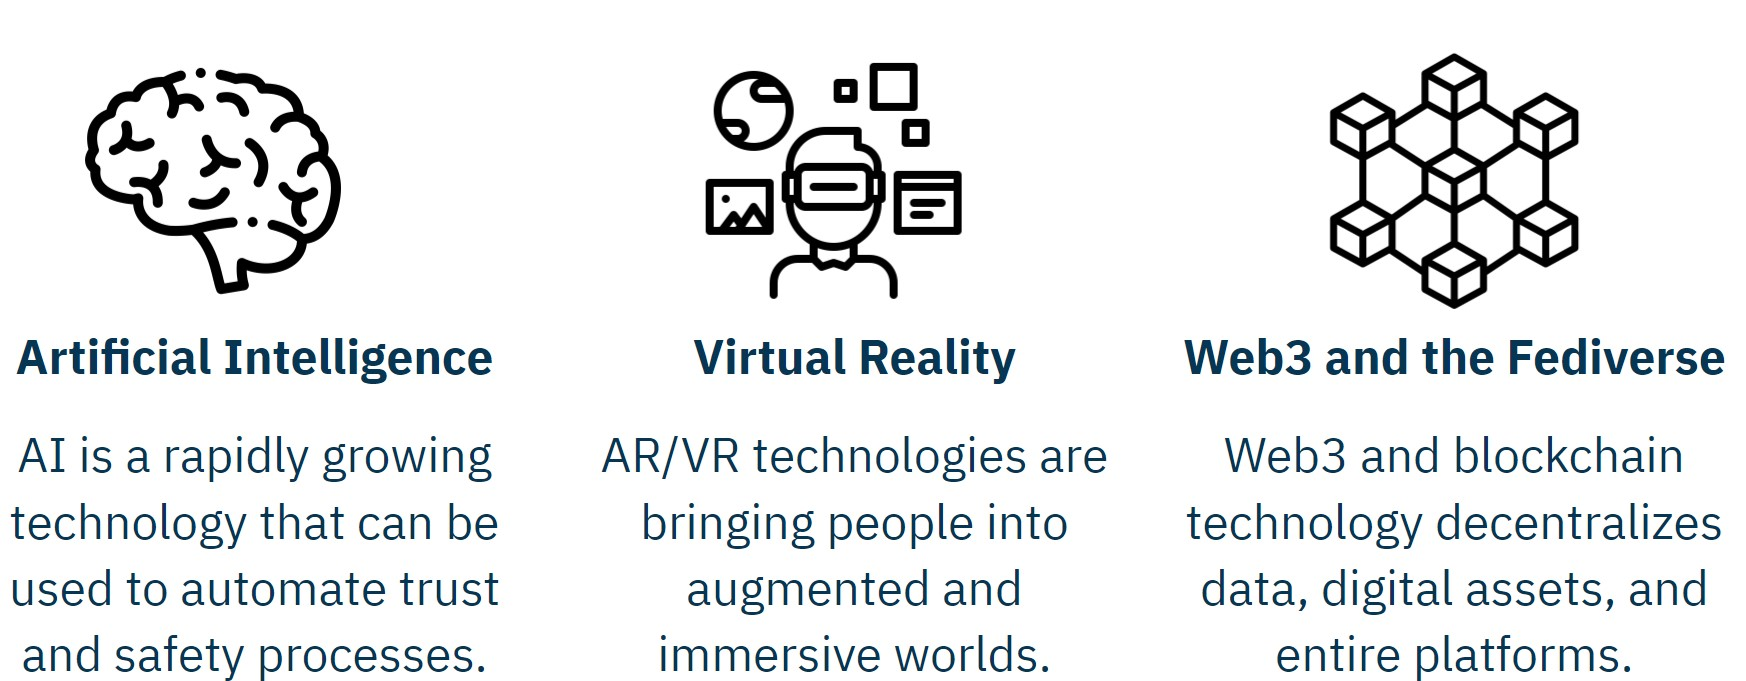
\includegraphics[width=\textwidth]{img/fig1.jpg}
\end{center}

\end{frame}


%%%%%%%%%%%%%%%%%%%%%%%%%%%%%%%%%%%%%%%%%%%%%%%%%%%
%%%%%%%%%%%%%%%%%%%% SLIDE 4 %%%%%%%%%%%%%%%%%%%%%%
%%%%%%%%%%%%%%%%%%%%%%%%%%%%%%%%%%%%%%%%%%%%%%%%%%%
\begin{frame}{}

\Huge{\textbf{Artificial Intelligence}}

\end{frame}



%%%%%%%%%%%%%%%%%%%%%%%%%%%%%%%%%%%%%%%%%%%%%%%%%%%
%%%%%%%%%%%%%%%%%%%% SLIDE 5 %%%%%%%%%%%%%%%%%%%%%%
%%%%%%%%%%%%%%%%%%%%%%%%%%%%%%%%%%%%%%%%%%%%%%%%%%%
\begin{frame}{What is Artificial Intelligence?}

\begin{center}
    \hspace*{-4ex}
    
\includegraphics[scale=.325]{img/fig2.jpg}
\end{center}

\note[]{AI System/Definitions (left) 
\begin{itemize}
    \item OECD (image from: \url{https://oecd.ai/en/wonk/cset-test-classification-ai-systems}
    \item Other key definitions from
    \begin{itemize}
        \item White House
        \item NIST \newline 
    \end{itemize}
\end{itemize} 

AI Definitions (right) 
\begin{itemize}
    \item CC license
    \item Image from this paper: \url{https://www.researchgate.net/figure/sualization-of-algorithms-vs-artificial-intelligence-vs-machine-learning-vs-deep_fig1_339997962}
\end{itemize}

}

\end{frame}



%%%%%%%%%%%%%%%%%%%%%%%%%%%%%%%%%%%%%%%%%%%%%%%%%%%
%%%%%%%%%%%%%%%%%%%% SLIDE 6 %%%%%%%%%%%%%%%%%%%%%%
%%%%%%%%%%%%%%%%%%%%%%%%%%%%%%%%%%%%%%%%%%%%%%%%%%%
\begin{frame}{What does AI have to do with Trust \& Safety?}

“Content moderation”, but to break that down.. 
\begin{itemize}
    \item Identifying and scoring content
    \item Flagging content for review
    \item Actioning content
    \item Assisting humans with decisions
\end{itemize}

But also: 
\begin{itemize}
    \item Content \emph{recommendation}
    \item Equity, fairness, ‘bias’/harm
    \item Generating synthetic content to test
    \item More than just ‘content’ \newline 
\end{itemize}

\begin{center}
    \textbf{Reactive} + \textbf{Proactive} Approaches
\end{center}

\end{frame}


%%%%%%%%%%%%%%%%%%%%%%%%%%%%%%%%%%%%%%%%%%%%%%%%%%%
%%%%%%%%%%%%%%%%%%%% SLIDE 7 %%%%%%%%%%%%%%%%%%%%%%
%%%%%%%%%%%%%%%%%%%%%%%%%%%%%%%%%%%%%%%%%%%%%%%%%%%
\begin{frame}{Example 1}

\begin{center}
    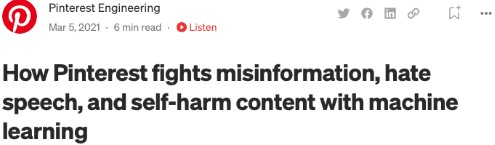
\includegraphics[width=.8\textwidth]{img/fig3.jpg}
\end{center}


\includegraphics[width=\textwidth]{img/fig4.jpg}

\note[]{From:\url{https://medium.com/pinterest-engineering/how-pinterest-fights-misinformation-hate-speech-and-self-harm-content-with-machine-learning-1806b73b40ef} \newline \newline 

Key points from post: 
\begin{itemize}
    \item Combination of ML + user reports
    \item Detect unsafe content before it’s reported
    \item Combination of methods, data sources signals
    \item Signals conveyed from keywords, images, etc
    \item Key questions around measurement
\end{itemize}
}

\end{frame}




%%%%%%%%%%%%%%%%%%%%%%%%%%%%%%%%%%%%%%%%%%%%%%%%%%%
%%%%%%%%%%%%%%%%%%%% SLIDE 8 %%%%%%%%%%%%%%%%%%%%%%
%%%%%%%%%%%%%%%%%%%%%%%%%%%%%%%%%%%%%%%%%%%%%%%%%%%
\begin{frame}{Example 2}

\hspace*{-7ex}
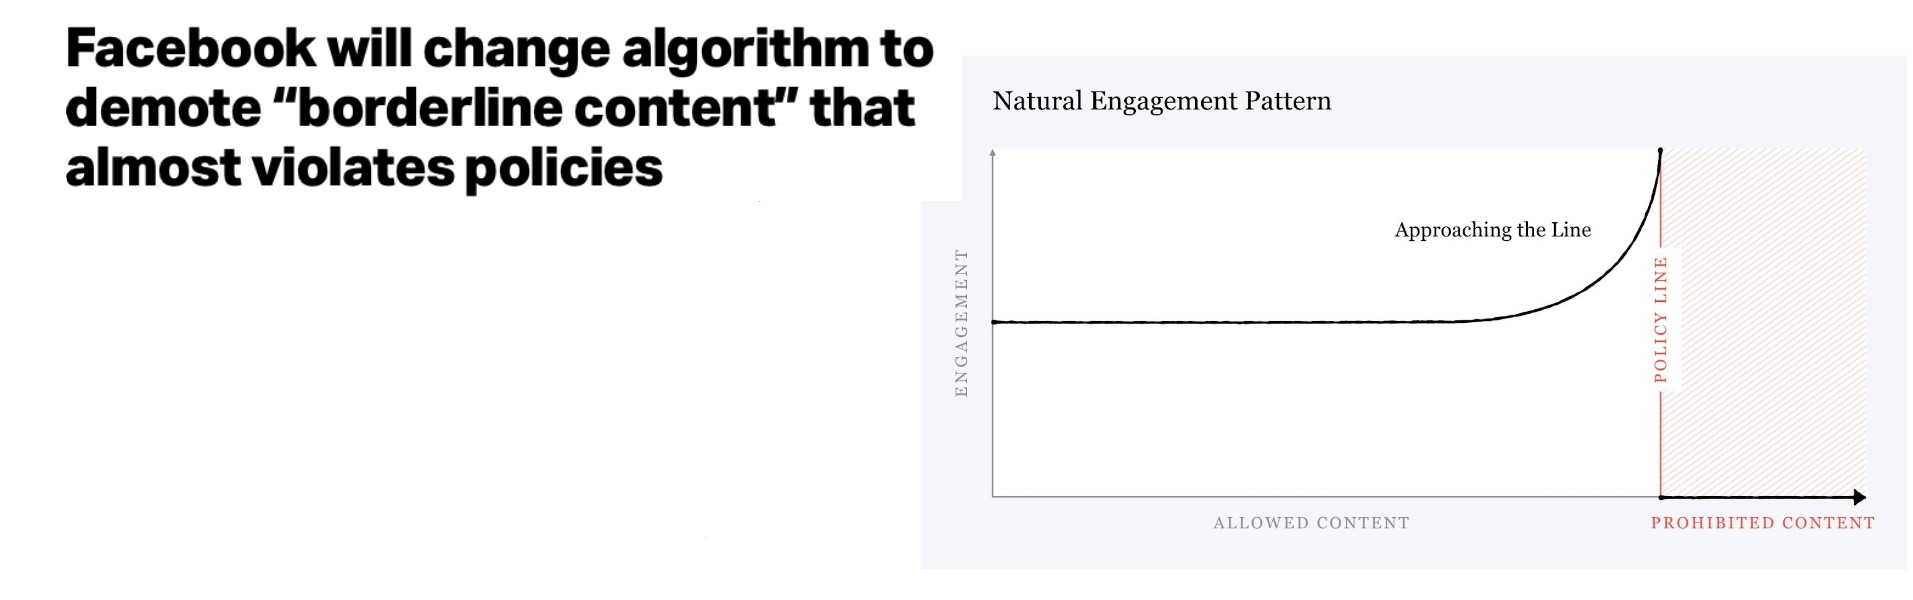
\includegraphics[scale=.32]{img/fig5.jpg}

\note[]{Usage of AI/ML to identify borderline content + prohibited content}

\end{frame}



%%%%%%%%%%%%%%%%%%%%%%%%%%%%%%%%%%%%%%%%%%%%%%%%%%%
%%%%%%%%%%%%%%%%%%%% SLIDE 9 %%%%%%%%%%%%%%%%%%%%%%
%%%%%%%%%%%%%%%%%%%%%%%%%%%%%%%%%%%%%%%%%%%%%%%%%%%
\begin{frame}{Interactive Demo/Breakout}

\hspace*{-6ex}
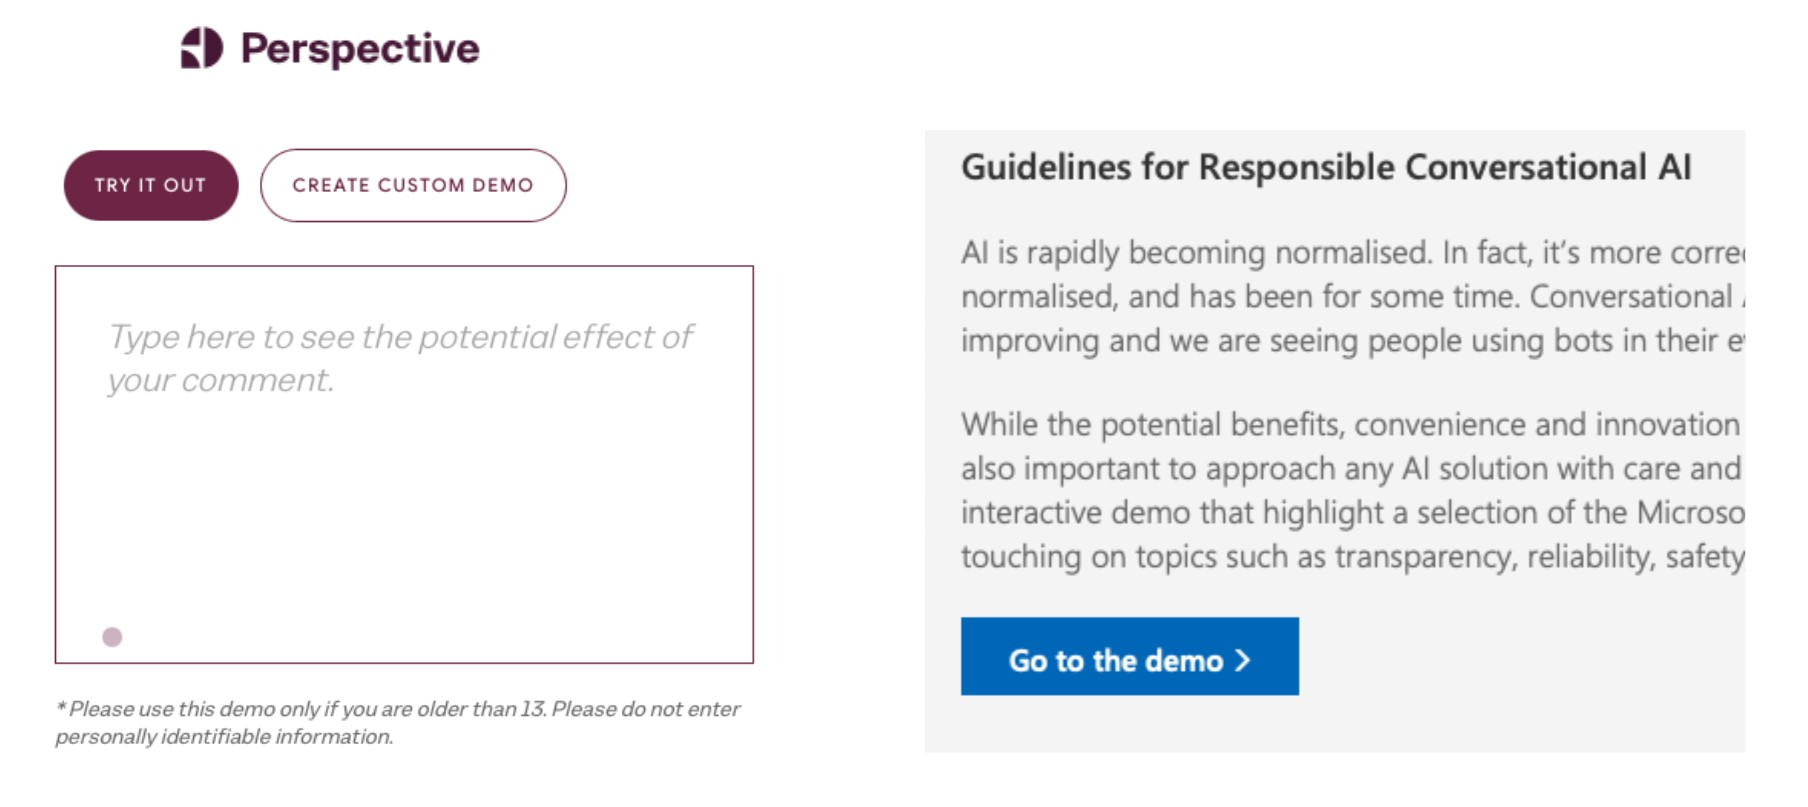
\includegraphics[scale=.34]{img/fig6.jpg}


\note[]{Try out one of these services/learning demos to learn more about: \newline 
\begin{itemize}
    \item Toxicity/harmful speech detection - \url{https://perspectiveapi.com/}
    \item MSFT conversational responsible AI demos
    \item \url{https://teachablemachine.withgoogle.com/}
\end{itemize}

}
\end{frame}




%%%%%%%%%%%%%%%%%%%%%%%%%%%%%%%%%%%%%%%%%%%%%%%%%%%
%%%%%%%%%%%%%%%%%%%% SLIDE 10 %%%%%%%%%%%%%%%%%%%%%%
%%%%%%%%%%%%%%%%%%%%%%%%%%%%%%%%%%%%%%%%%%%%%%%%%%%
\begin{frame}{Discussion Questions}

\begin{itemize}
    \item What types of T\&S-related topics can (and should) AI/ML based systems address?
    \item What is \emph{not} well suited to be addressed by AI or automated methods in T\&S?
    \item Policy development and enforcement often require judgements about context. What are important contextual signals that should be considered in human/machine environments?
    \item How would you measure the effectiveness of AI systems for T\&S objectives?
    \item How should T\&S practitioners think about differential impact across communities, including markets? Like those in the Global South, where training data may be less reflective of specific populations
\end{itemize}

\end{frame}



%%%%%%%%%%%%%%%%%%%%%%%%%%%%%%%%%%%%%%%%%%%%%%%%%%%
%%%%%%%%%%%%%%%%%%%% SLIDE 11 %%%%%%%%%%%%%%%%%%%%%%
%%%%%%%%%%%%%%%%%%%%%%%%%%%%%%%%%%%%%%%%%%%%%%%%%%%
\begin{frame}{}

\Huge{\textbf{Virtual and Augmented Reality}}

\note[]{\url{https://newpublic.substack.com/p/a-social-network-taxonomy}}
\end{frame}


%%%%%%%%%%%%%%%%%%%%%%%%%%%%%%%%%%%%%%%%%%%%%%%%%%%
%%%%%%%%%%%%%%%%%%%% SLIDE 12 %%%%%%%%%%%%%%%%%%%%%%
%%%%%%%%%%%%%%%%%%%%%%%%%%%%%%%%%%%%%%%%%%%%%%%%%%%
\begin{frame}{Defining Augmented and Virtual Reality}

\hspace*{-2ex}
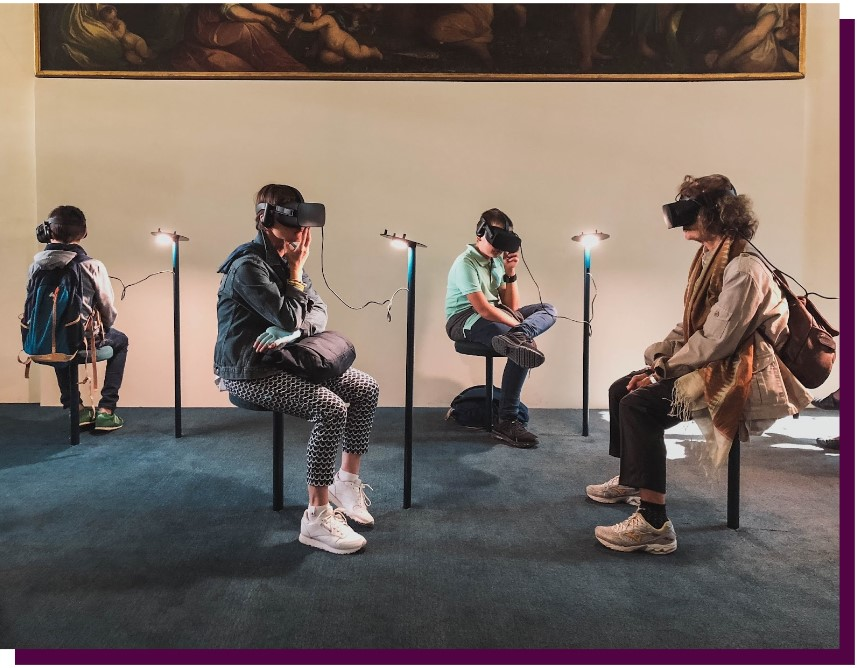
\includegraphics[width=.5\textwidth]{img/fig7.jpg}
\hfill 
\raisebox{-2ex}{
\begin{minipage}[b]{0.49\textwidth}
    \small{
        \begin{itemize} 
            \item \textbf{Augmented Reality} \newline Overlaying digital information onto the real world, typically through a device like a smartphone or a headset
            \item \textbf{Virtual Reality} \newline Fully immersive experiences in a simulated environment, typically through a dedicated VR headset
        \end{itemize}
    }
\end{minipage}
}
\end{frame}




%%%%%%%%%%%%%%%%%%%%%%%%%%%%%%%%%%%%%%%%%%%%%%%%%%%
%%%%%%%%%%%%%%%%%%%% SLIDE 13 %%%%%%%%%%%%%%%%%%%%%%
%%%%%%%%%%%%%%%%%%%%%%%%%%%%%%%%%%%%%%%%%%%%%%%%%%%
\begin{frame}{Example Harm Areas of AR and VR}

%\hspace*{-2ex}
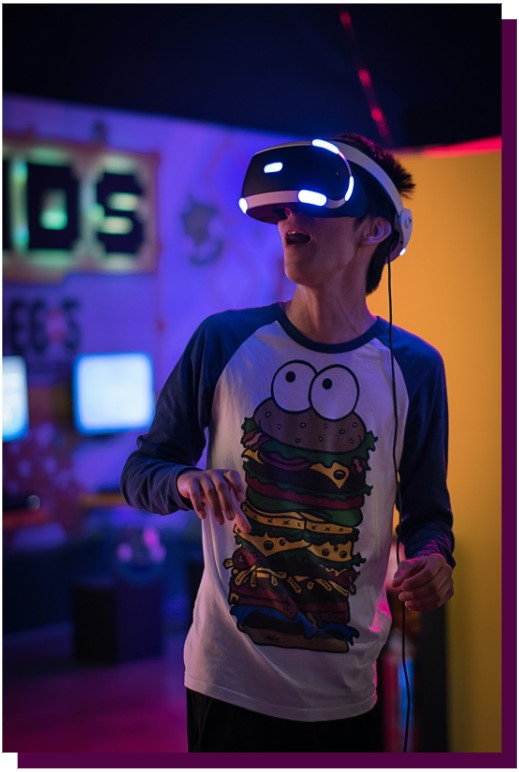
\includegraphics[scale = .4]{img/fig8.jpg}
\hfill
\raisebox{5ex}{
\begin{minipage}[b]{0.5\textwidth}
    \small{
        \raggedright 
        In immersive and augmented spaces, long-standing areas of harm take on new dimensions: 
        \begin{itemize} 
            \item Harassment and bullying
            \item Inappropriate content
            \item Privacy concerns
            \item Age restrictions and child safety
            \item Accessibility and inclusivity
        \end{itemize}
    }
\end{minipage}
}

\end{frame}





%%%%%%%%%%%%%%%%%%%%%%%%%%%%%%%%%%%%%%%%%%%%%%%%%%%
%%%%%%%%%%%%%%%%%%%% SLIDE 14 %%%%%%%%%%%%%%%%%%%%%%
%%%%%%%%%%%%%%%%%%%%%%%%%%%%%%%%%%%%%%%%%%%%%%%%%%%
\begin{frame}{Discussion Questions}

\small{
\begin{itemize}
    \item How do trust and safety concerns differ between virtual reality (VR), augmented reality (AR), and traditional digital environments? Discuss the unique challenges and opportunities that immersive technologies present for content moderation.
    \item What are the ethical considerations surrounding the collection and use of user data in VR and AR environments? How can platforms ensure that they respect user privacy while promoting safety?
    \item Discuss the role of AI and machine learning in moderating VR and AR experiences. What are the benefits and limitations of these technologies, and how can they aid human moderation?
    \item How can VR and AR platforms foster a culture of empathy, respect, and inclusivity among users? Discuss the role of virtual etiquette, social norms, and digital citizenship in creating a safe and welcoming environment for all users.
\end{itemize}
}

\end{frame}




%%%%%%%%%%%%%%%%%%%%%%%%%%%%%%%%%%%%%%%%%%%%%%%%%%%
%%%%%%%%%%%%%%%%%%%% SLIDE 15 %%%%%%%%%%%%%%%%%%%%%%
%%%%%%%%%%%%%%%%%%%%%%%%%%%%%%%%%%%%%%%%%%%%%%%%%%%
\begin{frame}{}

\Huge{\textbf{Decentralized Technologies}}

\end{frame}





%%%%%%%%%%%%%%%%%%%%%%%%%%%%%%%%%%%%%%%%%%%%%%%%%%%
%%%%%%%%%%%%%%%%%%%% SLIDE 16 %%%%%%%%%%%%%%%%%%%%%%
%%%%%%%%%%%%%%%%%%%%%%%%%%%%%%%%%%%%%%%%%%%%%%%%%%%
\begin{frame}{Blockchain, Cryptocurrencies, NFTs}

Web3 and blockchain technology provides a decentralized way to structure platforms, data, and digital currencies. \newline 

It can also be used to create and manage ownership of digital assets that are used on tech platforms and even in-game experiences. \newline 

These novel technologies also introduce new abuse vectors that you may face as a Trust \& Safety professional.


\end{frame}




%%%%%%%%%%%%%%%%%%%%%%%%%%%%%%%%%%%%%%%%%%%%%%%%%%%
%%%%%%%%%%%%%%%%%%%% SLIDE 17 %%%%%%%%%%%%%%%%%%%%%%
%%%%%%%%%%%%%%%%%%%%%%%%%%%%%%%%%%%%%%%%%%%%%%%%%%%
\begin{frame}{Blockchain, Cryptocurrencies, NFTs}

    \begin{itemize}
        \item \textbf{Blockchain Technology} provides a decentralized and secure way to store data and conduct transactions.
        \item \textbf{Key Attributes} 
        \begin{itemize}
            \item Decentralization
            \item Encryption
            \item Consensus mechanisms
        \end{itemize}
        \item \textbf{Cryptocurrency} Digital or virtual currency that uses cryptography for security and operates on a decentralized network.
        \item \textbf{NFTs} 
        ‘Non-Fungible Tokens’, or  a digital asset with a unique identifier.
    \end{itemize}


\end{frame}


%%%%%%%%%%%%%%%%%%%%%%%%%%%%%%%%%%%%%%%%%%%%%%%%%%%
%%%%%%%%%%%%%%%%%%%% SLIDE 18 %%%%%%%%%%%%%%%%%%%%%%
%%%%%%%%%%%%%%%%%%%%%%%%%%%%%%%%%%%%%%%%%%%%%%%%%%%
\begin{frame}{Blockchain, Cryptocurrencies, NFTs}

\hspace*{-2ex}
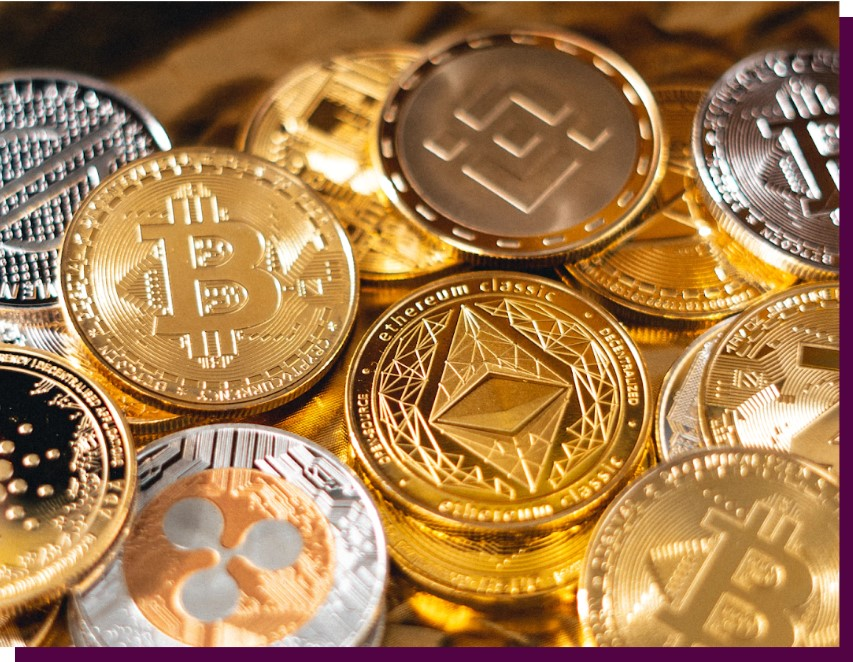
\includegraphics[width=.5\textwidth]{img/fig9.jpg}
\hfill 
\begin{minipage}[b]{0.49\textwidth}
    \small{
    Example Technologies:
        \begin{itemize} 
            \item \textbf{Cryptocurrency:} Digital or virtual currency that uses cryptography for security and operates on a decentralized network.
            \item  \textbf{NFTs:} ‘Non-Fungible Tokens’, or  a digital asset with a unique identifier.
        \end{itemize}
    }
\end{minipage}

\end{frame}




%%%%%%%%%%%%%%%%%%%%%%%%%%%%%%%%%%%%%%%%%%%%%%%%%%%
%%%%%%%%%%%%%%%%%%%% SLIDE 19 %%%%%%%%%%%%%%%%%%%%%%
%%%%%%%%%%%%%%%%%%%%%%%%%%%%%%%%%%%%%%%%%%%%%%%%%%%
\begin{frame}{Blockchain, Cryptocurrencies, NFTs}

%\hspace*{-2ex}
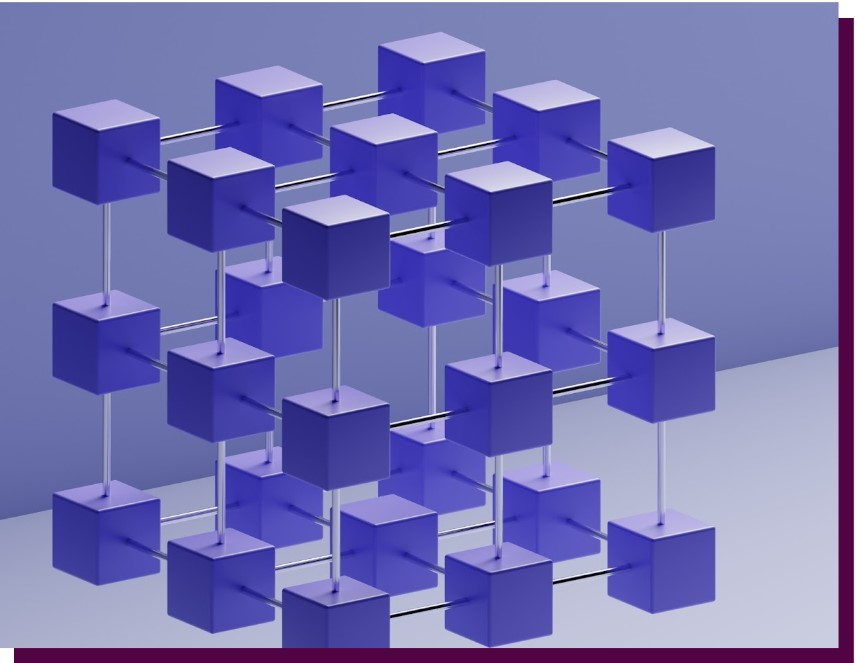
\includegraphics[width=.50\textwidth]{img/fig10.jpg}
\hfill 
\raisebox{-2ex}{
\begin{minipage}[b]{0.47\textwidth}
    \small{
        \begin{itemize} 
            \item Decentralization can raise major harm vectors, including: 

            \begin{itemize}
                \item Account Stealing and other platform integrity vulnerabilities
                \item Financial Fraud and Scams
                \item Inauthentic Behavior
                \item Social Engineering
            \end{itemize}
        \end{itemize}
    }
\end{minipage}
}

\end{frame}


%%%%%%%%%%%%%%%%%%%%%%%%%%%%%%%%%%%%%%%%%%%%%%%%%%%
%%%%%%%%%%%%%%%%%%%% SLIDE 20 %%%%%%%%%%%%%%%%%%%%%%
%%%%%%%%%%%%%%%%%%%%%%%%%%%%%%%%%%%%%%%%%%%%%%%%%%%
\begin{frame}{Discussion Questions}

\footnotesize{

\begin{itemize}
    \item How do trust and safety concerns manifest in the context of cryptocurrencies, NFTs, and digital assets? Discuss the unique challenges these technologies present compared to traditional financial systems and assets.
    \item Explore the potential risks associated with the use of cryptocurrencies and NFTs, such as fraud, money laundering, and illicit activities. How can these risks be mitigated while preserving the benefits of decentralization and user autonomy?
    \item Discuss the role of self-regulation in the cryptocurrency and NFT ecosystem. How can industry stakeholders, such as exchanges, wallet providers, and developers, contribute to trust and safety?
    \item Analyze the implications of content moderation for NFTs and digital assets, particularly in relation to intellectual property rights, copyright infringement, and counterfeit goods. How can platforms balance free expression with the protection of creators' rights?
    \item Discuss the importance of user education and awareness in promoting trust and safety in the cryptocurrency and NFT space. How can platforms, developers, and regulators collaborate to empower users to make informed decisions?
\end{itemize}
}
\end{frame}




%%%%%%%%%%%%%%%%%%%%%%%%%%%%%%%%%%%%%%%%%%%%%%%%%%%
%%%%%%%%%%%%%%%%%%%% SLIDE 21 %%%%%%%%%%%%%%%%%%%%%%
%%%%%%%%%%%%%%%%%%%%%%%%%%%%%%%%%%%%%%%%%%%%%%%%%%%
\begin{frame}{The Fediverse}

The advent of new technologies includes converging with what has come so far.  Platforms still create opportunities to create content, but now they’re federated across different servers. \newline 

Content, games, art, and currency is built on the blockchain. Ownership is in the hands of users, granting greater user freedoms and ownership, and challenging traditional models of keeping platforms safe. \newline 

In this section, we go over some of the promises and challenges of decentralized technologies.

\end{frame}





%%%%%%%%%%%%%%%%%%%%%%%%%%%%%%%%%%%%%%%%%%%%%%%%%%%
%%%%%%%%%%%%%%%%%%%% SLIDE 22 %%%%%%%%%%%%%%%%%%%%%%
%%%%%%%%%%%%%%%%%%%%%%%%%%%%%%%%%%%%%%%%%%%%%%%%%%%
\begin{frame}{Fediverse}

\begin{minipage}[]{0.53\textwidth}
    \small{
    \begin{itemize}
        \item \textbf{What does it mean to be “Federated”?}

        \begin{itemize}
            \item Decentralized and interoperable network of independent social media platforms.
            \item Communicate using open-source protocols. 
            \item Enables users to join various self-hosted instances or servers.
        \end{itemize}
    \end{itemize}
    }
\end{minipage}
\hfill
\begin{minipage}[]{0.46\textwidth}
    \small{
    \begin{itemize}
        \item \textbf{Moderation}

        \begin{itemize}
            \item Usually team of volunteer moderators and administrators.
            \item Set policies and enforce them within federated instance/server.
        \end{itemize}
    \end{itemize}

    \begin{itemize}
        \item \textbf{Example Platforms}

        \begin{itemize}
            \item Mastodon
            \item Funkwhale
            \item diaspora*
        \end{itemize}
    \end{itemize}
    }
\end{minipage}

\end{frame}





%%%%%%%%%%%%%%%%%%%%%%%%%%%%%%%%%%%%%%%%%%%%%%%%%%%
%%%%%%%%%%%%%%%%%%%% SLIDE 23 %%%%%%%%%%%%%%%%%%%%%%
%%%%%%%%%%%%%%%%%%%%%%%%%%%%%%%%%%%%%%%%%%%%%%%%%%%
\begin{frame}{Fediverse and Content Moderation}
 
\vspace*{3ex}
\raisebox{2.7ex}{
\begin{minipage}[b]{0.43\textwidth}
    \small{
        \begin{itemize} 
            \item Fediverse communities are governed by administrators or moderators
            \item Similar to internet forums, community platforms (e.g. Facebook Pages, Reddit subreddits, Discord servers)
            \item What’s different? There’s a limited centralized Trust \& Safety function
        \end{itemize}
    }
\end{minipage}}
\hfill
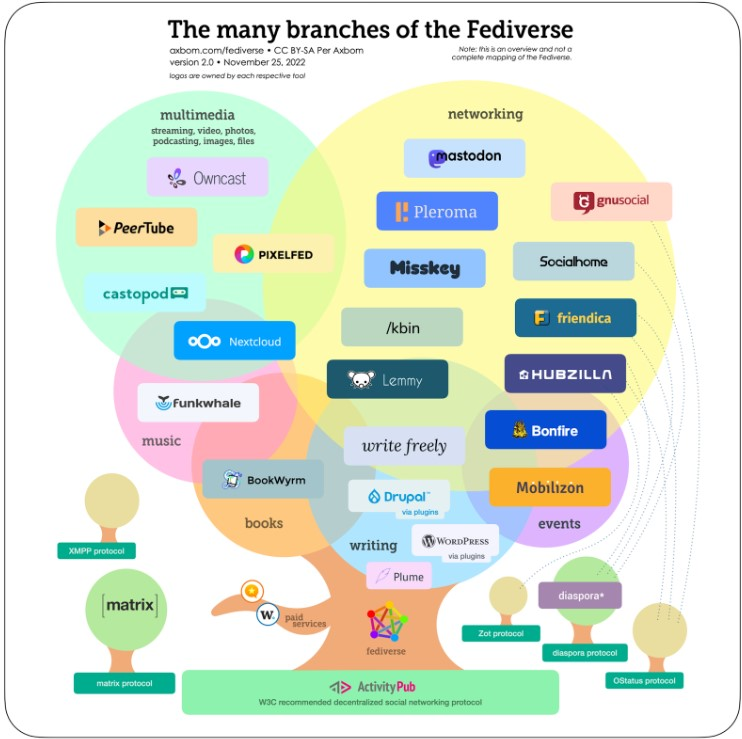
\includegraphics[width=.54\textwidth]{img/fig11.jpg}

\end{frame}





%%%%%%%%%%%%%%%%%%%%%%%%%%%%%%%%%%%%%%%%%%%%%%%%%%%
%%%%%%%%%%%%%%%%%%%% SLIDE 24 %%%%%%%%%%%%%%%%%%%%%%
%%%%%%%%%%%%%%%%%%%%%%%%%%%%%%%%%%%%%%%%%%%%%%%%%%%
\begin{frame}{Discussion Questions}

\small{
\begin{itemize}
    \item What are the unique challenges of moderating content on a federated platform compared to centralized platforms? Discuss the advantages and disadvantages of both systems.
    \item Discuss the role of human moderators and automated systems in maintaining trust and safety on federated platforms. How can these two approaches complement each other?
    \item Analyze the concept of content moderation within the context of free speech and censorship. To what extent should federated platforms moderate content, and what principles should guide their decisions?
    \item What are the potential risks associated with self-governance on federated platforms? How can these platforms mitigate these risks while preserving user autonomy?
    \item Discuss the potential legal and ethical implications of content moderation on federated platforms. How should these platforms navigate issues related to privacy, data protection, and liability?
\end{itemize}
}


\end{frame}



%%%%%%%%%%%%%%%%%%%%%%%%%%%%%%%%%%%%%%%%%%%%%%%%%%%
%%%%%%%%%%%%%%%%%%%% SLIDE 25 %%%%%%%%%%%%%%%%%%%%%%
%%%%%%%%%%%%%%%%%%%%%%%%%%%%%%%%%%%%%%%%%%%%%%%%%%%
\begin{frame}{}

\Huge{\textbf{Career Advice}}

\end{frame}




%%%%%%%%%%%%%%%%%%%%%%%%%%%%%%%%%%%%%%%%%%%%%%%%%%%
%%%%%%%%%%%%%%%%%%%% SLIDE 26 %%%%%%%%%%%%%%%%%%%%%%
%%%%%%%%%%%%%%%%%%%%%%%%%%%%%%%%%%%%%%%%%%%%%%%%%%%
\begin{frame}{Careers in Trust \& Safety}

In industry, Trust \& Safety professionals are responsible for ensuring the safety of users and clients in the policies they form, products they build, and stories they tell in telling an organization's story to the world. \newline

As new technologies emerge and novel forms of harm proliferate,  the impact of Trust \& Safety work will be more important than ever.


\end{frame}


%%%%%%%%%%%%%%%%%%%%%%%%%%%%%%%%%%%%%%%%%%%%%%%%%%%
%%%%%%%%%%%%%%%%%%%% SLIDE 27 %%%%%%%%%%%%%%%%%%%%%%
%%%%%%%%%%%%%%%%%%%%%%%%%%%%%%%%%%%%%%%%%%%%%%%%%%%
\begin{frame}{Trust \& Safety Roles in Tech}

\begin{center}
    
\includegraphics[width=.55\textwidth]{img/fig12.jpg}
\end{center}
    \footnotesize{
        \begin{itemize} 
            \item \textbf{Legal:} Guide company across teams on risk mitigation, develop responses to regulatory bodies and law enforcement.
            \item \textbf{Policy:} Design content policies, performing risk assessments for product teams, and forming partnerships with civil society and governments.
            \item \textbf{Operations:} Enforce policy through scaled operational programs. Dedicated teams across subject-matter expertise, program and project management.
        \end{itemize}
    }

\end{frame}



%%%%%%%%%%%%%%%%%%%%%%%%%%%%%%%%%%%%%%%%%%%%%%%%%%%
%%%%%%%%%%%%%%%%%%%% SLIDE 28 %%%%%%%%%%%%%%%%%%%%%%
%%%%%%%%%%%%%%%%%%%%%%%%%%%%%%%%%%%%%%%%%%%%%%%%%%%
\begin{frame}{Trust \& Safety Roles in Tech}

\begin{center}
    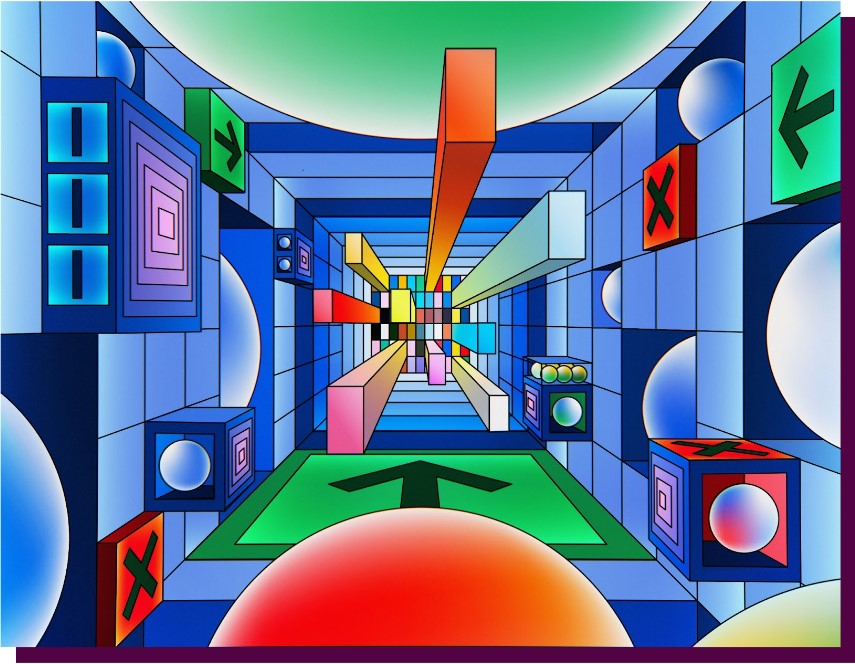
\includegraphics[width=.55\textwidth]{img/fig13.jpg}
\end{center}
    \footnotesize{
        \begin{itemize} 
            \item \textbf{Product \& Engineering:} Builds internal and consumer-facing products, including T\&S tooling to safety features
            \item \textbf{Data Science:} Analyzes policy violations and their impact on platforms, develops measurement and detection methods, and create strategies to address harms.
            \item \textbf{Marketing \& Communications:} Develops narrative strategies for showcasing organization's safety commitments. Drives content strategies and user research efforts.
        \end{itemize}
    }
\end{frame}



%%%%%%%%%%%%%%%%%%%%%%%%%%%%%%%%%%%%%%%%%%%%%%%%%%%
%%%%%%%%%%%%%%%%%%%% SLIDE 29 %%%%%%%%%%%%%%%%%%%%%%
%%%%%%%%%%%%%%%%%%%%%%%%%%%%%%%%%%%%%%%%%%%%%%%%%%%
\begin{frame}{Trust \& Safety Partnerships}

Working in Trust \& Safety doesn’t have to be limited to working at a tech company. \newline 

In fact, tech companies need extensive collaborations and partnerships across industry, academic, civil society, and government partners. 


\end{frame}



%%%%%%%%%%%%%%%%%%%%%%%%%%%%%%%%%%%%%%%%%%%%%%%%%%%
%%%%%%%%%%%%%%%%%%%% SLIDE 30 %%%%%%%%%%%%%%%%%%%%%%
%%%%%%%%%%%%%%%%%%%%%%%%%%%%%%%%%%%%%%%%%%%%%%%%%%%
\begin{frame}{Industry Partnerships}

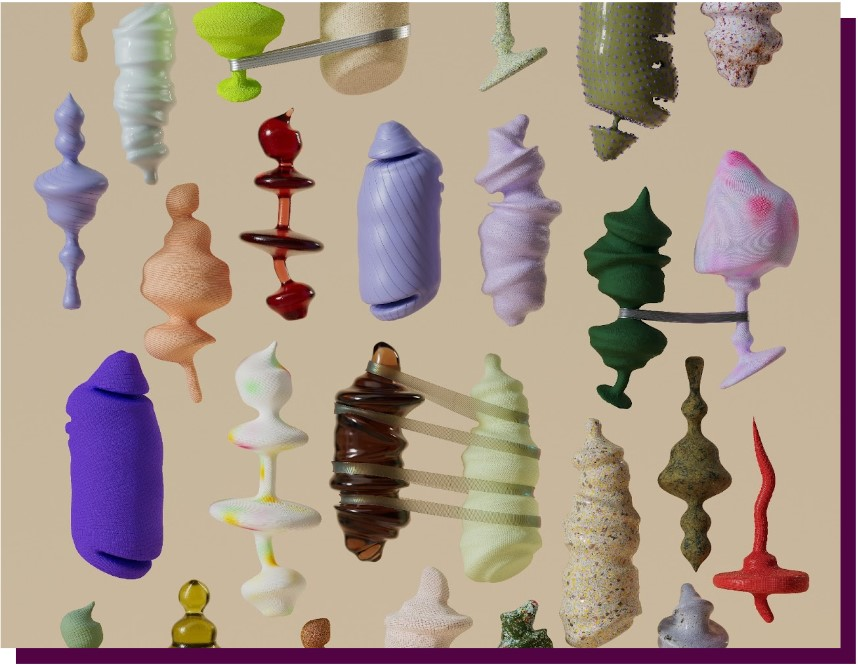
\includegraphics[width=.5\textwidth]{img/fig14.jpg}
\hfill
\begin{minipage}[b]{0.48\textwidth}
    \small{
        \begin{itemize} 
            \item Fellow tech companies and industry working groups
            \item Coordinate on operations and investigations
            \item Collaborate in industry working groups (e.g. TSPA) and share best practices
            \item Collaborate on guiding regulators
        \end{itemize}
    }
\end{minipage}

\end{frame}


%%%%%%%%%%%%%%%%%%%%%%%%%%%%%%%%%%%%%%%%%%%%%%%%%%%
%%%%%%%%%%%%%%%%%%%% SLIDE 31 %%%%%%%%%%%%%%%%%%%%%%
%%%%%%%%%%%%%%%%%%%%%%%%%%%%%%%%%%%%%%%%%%%%%%%%%%%
\begin{frame}{Academic Partnerships}

\begin{center}
    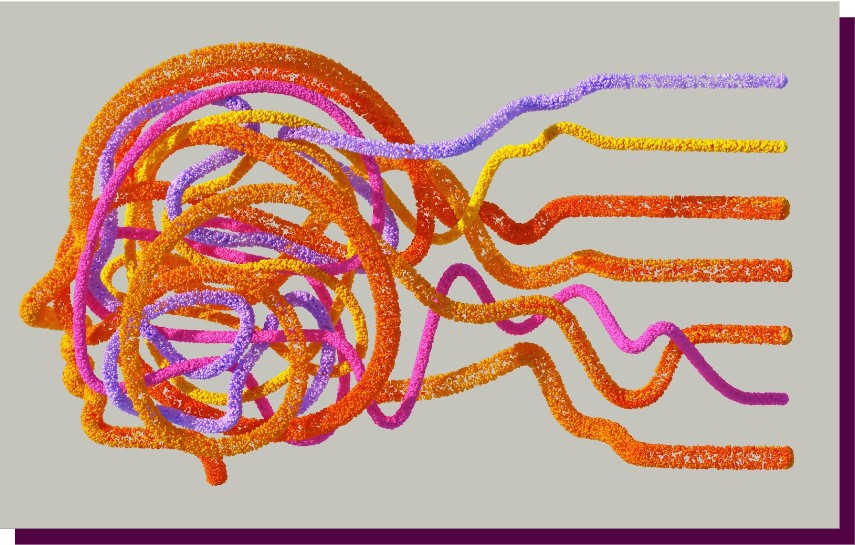
\includegraphics[width=.7\textwidth]{img/fig15.jpg}
\end{center}

\small{
    \begin{itemize} 
        \item Partner on user research and social impact 
        \item Guide product teams
        \item Audit content policies and public policy initiatives
        \item Example partners: academic labs, PhD and Masters students, specialized researchers and research projects
    \end{itemize}
}
\end{frame}




%%%%%%%%%%%%%%%%%%%%%%%%%%%%%%%%%%%%%%%%%%%%%%%%%%%
%%%%%%%%%%%%%%%%%%%% SLIDE 32 %%%%%%%%%%%%%%%%%%%%%%
%%%%%%%%%%%%%%%%%%%%%%%%%%%%%%%%%%%%%%%%%%%%%%%%%%%
\begin{frame}{Civil Society Partnerships}
\vspace*{4ex}
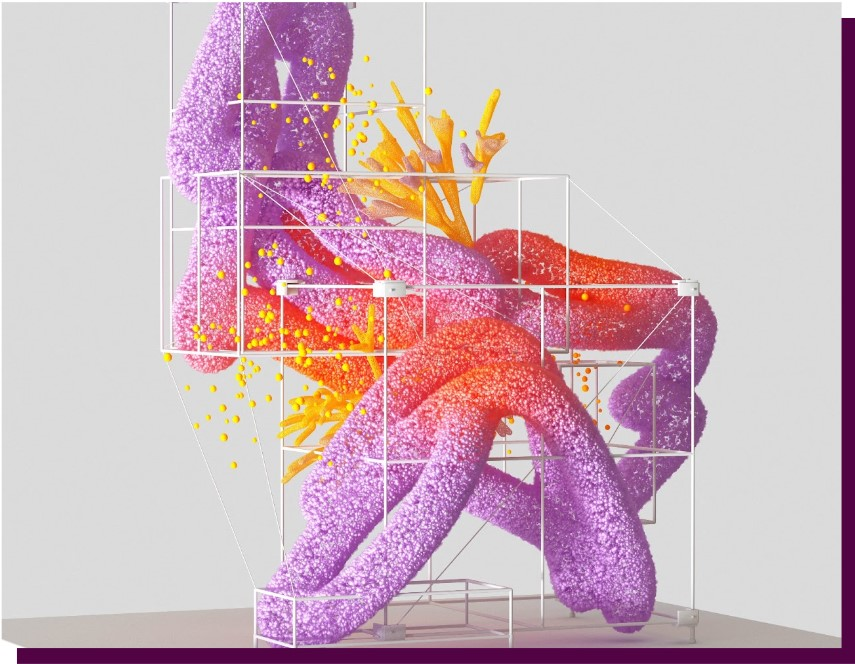
\includegraphics[width=.52\textwidth]{img/fig16.jpg}
\hfill
\raisebox{5ex}{
\begin{minipage}[]{0.45\textwidth}
    \small{
        \begin{itemize} 
            \item Create guiding frameworks for policy, product, data privacy, Trust \& Safety operations
            \item Co-create education resources and industry reports to guide industry awareness of issues
            \item Example Partners: subject-matter focused (e.g. child safety), product-based (e.g. organizations developing AI product and policy frameworks)
        \end{itemize}
    }
\end{minipage}}
\end{frame}


%%%%%%%%%%%%%%%%%%%%%%%%%%%%%%%%%%%%%%%%%%%%%%%%%%%
%%%%%%%%%%%%%%%%%%%% SLIDE 33 %%%%%%%%%%%%%%%%%%%%%%
%%%%%%%%%%%%%%%%%%%%%%%%%%%%%%%%%%%%%%%%%%%%%%%%%%%
\begin{frame}{Governments}

\begin{center}
    
\includegraphics[width=.7\textwidth]{img/fig17.jpg}
\end{center}

\small{
    \begin{itemize} 
        \item Regulate platform content moderation practices and safety   products
        \item Issue law enforcement inquiries (e.g. subpoenas, exigent requests)
        \item Example partners: local, provincial, national, and international governing bodies, law enforcement agencies
    \end{itemize}
}
\end{frame}





%%%%%%%%%%%%%%%%%%%%%%%%%%%%%%%%%%%%%%%%%%%%%%%%%%%
%%%%%%%%%%%%%%%%%%%% SLIDE 34 %%%%%%%%%%%%%%%%%%%%%%
%%%%%%%%%%%%%%%%%%%%%%%%%%%%%%%%%%%%%%%%%%%%%%%%%%%
\begin{frame}{Readings / References}

\begin{itemize}
    \item \href{https://www.flaticon.com/free-icons/blockchain}{Blockchain} icon created by Good Ware
    \item \href{https://www.flaticon.com/free-icons/brain}{Brain icon} created by Freepik 
    \item \href{https://www.flaticon.com/free-icons/vr}{VR} icon created by Nikita Golubev
    \item Fediverse map by Per Axbom, \url{https://axbom.com/fediverse/}
    \item Career Advice section art from DeepMind’s Visualising AI project, \url{https://visualisingai.deepmind.com}
\end{itemize}

\end{frame}
%\backpage

\end{document}